\documentclass{article}
% translate with >> pdflatex -shell-escape <file>

\usepackage{pgfplots}
\pgfplotsset{compat=newest}

\pagestyle{empty}

\begin{document}
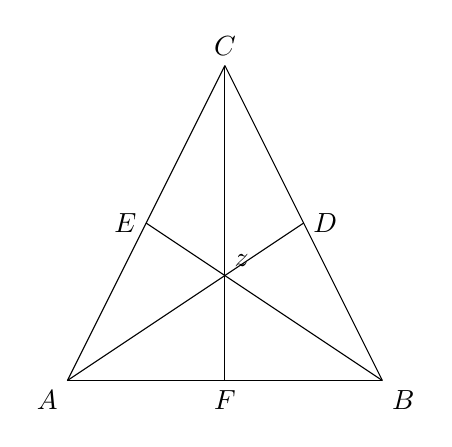
\begin{tikzpicture}%
    \draw (-2, 0) -- (2, 0) (-2, 0) node[anchor = north east] {$A$};
    \draw (2, 0) -- (0, 4) (2, 0) node[anchor = north west] {$B$};
    \draw (-2, 0) -- (0, 4) (0, 4) node[anchor = south] {$C$};
    \draw (2, 0) -- (-1, 2) (-1, 2) node[anchor = east] {$E$};
    \draw (0, 4) -- (0, 0) (0, 0) node[anchor = north] {$F$};
    \draw (-2, 0) -- (1, 2) (1, 2) node[anchor = west] {$D$};
    \draw (0, 1.33) node[anchor= south west] {$z$};
\end{tikzpicture}%
\end{document}

